
In diesem Kapitel wird zunächst auf die Implementierung von SIBs im allgemeinen eingegangen.
Darauf folgt die genaue Beschreibung der für das Projekt erstellten SIBs, sowie die Darstellung zweier
 Besonderheiten im diesem Entwicklungsprozess.
\FloatBarrier
\subsubsection{Allgemeines zur SIB-Programmierung}
Im jABC können SIBs über eine Baumstruktur ausgewählt und dann bequem in das Prozessmodell eingebunden werden.
Um die verwendeten SIBs miteinander zu verbinden, besitzt jedes SIB fest definierte ausgehende Kanten, im
 jABC-Kontext auch Branches genannt. Zudem ist es üblich, dass ein SIB definierte Parameter benötigt, um dessen
 Ausführung zu steuern.
Je nach Zweck des einzelnen SIB unterscheiden sich daher dessen Branches und Parameter.
Im folgenden wird nun erläutert, wie ein solches SIB erstellt wird.

Da jABC eine Java-Anwendung ist und die Ausführung des Prozessmodells, und dadurch auch die Ausführung der
 einzelnen SIBs an sich, innerhalb von jABC stattfindet, werden die einzelnen SIBs ebenfalls in Java implementiert.
Ein SIB wird dabei durch eine Java-Klasse repräsentiert, welche mit der Annotation \lstinline{@SIBClass} versehen ist.
Durch diese Annotation wird die Java-Klasse von jABC als SIB erkannt.

Damit das SIB innerhalb einer Modellausführung verwendet werden kann, müssen jedoch zunächst noch Branches und
 Parameter definiert werden. Mögliche Branches werden dabei über eine öffentliche Klassenvariable namens \lstinline{BRANCHES}
 definiert, welche vom Typ \lstinline{String[]}-Array ist.
Auch SIB-Parameter sind öffentliche Klassenvariablen.
Der Name der Variablen ist beliebig und es kann aus den üblichen Standard-Typen (z.B. \lstinline{boolean}, \lstinline{int},
 \lstinline{String}, ...) ausgewählt werden.
 Für die Notwendigkeit der Anwendung von komplizierteren Parametern, wie ganzen Klassen, stellt jABC den Variablentyp
  \lstinline{ContextKey} zur Verfügung.
 Mit diesem ist es möglich Objekte innerhalb des Ausführungskontextes von jABC zu referenzieren.
 Diese können dann lesend wie schreibend verwendet werden.
 In jABC ist der Ausführungskontext über eine \lstinline{Map} realisiert.
 Daher auch der Name \lstinline{ContextKey} des Variablentyps, denn bei der Deklaration einer Variable von diesem Typ ist
  lediglich der zugehörige Schlüssel aus der \lstinline{Map} anzugeben.
 Die Klassenvariable kann dann dazu verwendet werden, auf die Daten im Ausführungskontext zuzugreifen.

Jedoch bedarf es noch einer weiteren Ergänzung, um ein SIB vollständig zu implementieren.
Es muss noch definiert werden, was dieses SIB eigentlich tun soll.
Hierfür muss die Java-Klasse des SIBs das Interface \lstinline{Executable} implementieren, welches verlangt,
 dass die Klasse die Methode \lstinline{trace()} definiert. Diese Methode \lstinline{trace()} wird innerhalb von jABC
 in dem Moment aufgerufen, wenn die Ausführung des SIBs beginnen soll.
Als Parameter wird eine Variable vom Typ \lstinline{ExecutionEnvironment} übergeben, welche für den Zugriff auf den
 Ausführungskontext erforderlich ist.
Zuletzt muss jABC noch mitgeteilt werden, welcher Branch im Anschluss an die Ausführung gewählt werden soll.
Die Methode \lstinline{trace()} besitzt hierzu den Rückgabewert \lstinline{String}.
Überlicherweise wird der Rückgabewert aus dem wie oben definierten \lstinline{String[]}-Array \lstinline{BRANCHES} ausgewählt.

Das \autoref{lst:samplesib} zeigt exemplarisch den Kopf einer typischen Implementierung einer SIB-Klasse.

% Listing SIB-Klasse %
\javalstset{MySIB}{lst:samplesib}
\begin{lstlisting}[float=h!t]
@SIBClass("My-SIB")
public class MySib implements Executable {

	// Branches
    public final String[] BRANCHES = {"default", "error"};

    // Parameter
    public \lstinline{ContextKey} someKey = new ContextKey("someKey");
    public String title = "Nice Title";

    @Override
    public String trace(ExecutionEnvironment env) {
        ...
		return "default";
    }
	...
}
\end{lstlisting}

% Listing SIB-Klasse ENDE %
\FloatBarrier
\subsubsection{Spezifikation notwendiger SIBs}
Wie bereits aus der Projektstruktur in Abbildung \ref{fig:projektaufbau} ersichtlich, sind verschiedene Arten von SIBs
 für ein geeignetes Modell notwendig.
Zum einen werden SIBs benötigt, welche die Funktionen der Konnektoren benutzen.
Zum anderen müssen SIBs implementiert werden, welche über GUI-Elemente die Eingaben des Nutzers abfragen.
Daraus ergibt sich die Notwendigkeit folgender SIBs.

Ein zentrales Element des Prozessen ist die Suche nach Kontakten anhand gegebener Kriterien.
Daher werden für die beiden Suchfunktionen (bei SAP und Google) passend zwei SIBs implementiert.
Die beiden SIBs unterscheiden sich jedoch nur in der Form, dass sie bei der Ausführung die jeweils passende Suchmethode
 der externen Datenbank verwenden.
Äußerlich unterscheiden sich diese, bis auf den Namen, daher nicht.
Als Eingabe erwarten beide Suchfunktionen einen Parameter vom Typ des in der Einleitung beschriebenen \lstinline{Contact}-Objektes.
Zurück liefern beide Funktionen eine Liste von eben genannten \lstinline{Contact}-Objekten. Parameter und Rückgabewert
 sind als SIB-Parameter vom Typ \lstinline{ContextKey} implementiert, wodurch eine weitere Verwendung möglich wird.
Definierte Branches der beiden SIBs sind \emph{found} (für den Fall dass die zurückgelieferte Liste nicht leer ist),
 \emph{not found} (im Falle einer leeren Rückgabeliste) und \emph{error} (wird gewählt, wenn die Ausführung der
 Suchfunktion eine \lstinline{Exception} wirft).\\

Ein weiteres Element einer Datenmigration ist das Hinzufügen der Objekte auf dem Zielsystem.
Zu diesem Zweck muss ein SIB erzeugt werden, welches die passende Funktion nutzt, um Kontakte dem Google-System hinzuzufügen.
Der Parameter des SIB ist in diesem Fall vom Typ \lstinline{ContextKey} und verweist auf ein \lstinline{Contact}-Objekt,
 dessen Variablen mit passenden Werten belegt sind.
Ein spezieller Rückgabewert ist in diesem Fall unnötig, denn Erfolg oder Misserfolg der Funktionsausführung wird über
 den gewählten Branch kommuniziert.
Zu diesem Zweck besitzt das SIB die zwei Branches \emph{default} (falls kein Fehler auftritt) und \emph{error} (falls
 \lstinline{Exception} geworfen wird, s.o.).

Damit ist die Kommunikation zu den externen Datenbanken ausreichen spezifiziert und es folgt die Definition der SIBs,
 welche für die Nutzereingaben verantwortlich sind.

Damit der Nutzer eine Suchanfrage definieren kann, muss jener die Daten eingeben können.
Hierzu wird ein SIB generiert, welches ein Fenster (Swing-Frame) öffnet und anschließend auf die Eingabe des Nutzers wartet.
Die Eingabefelder können mit den Werten eines \lstinline{Contact}-Objektes vorbelegt werden.
Wenn die Eingabe beendet ist, speichert das SIB die Daten in den Ausführungs"=kontext.
Zu diesem Zweck wurde ein passender SIB-Parameter vom Typ \lstinline{ContextKey} definiert.
Dieser dient sowohl für die Vorbelegung, als auch zur Speicherung der Eingaben.
Um die Wiederverwendbarkeit zu ermöglichen, wurde das SIB um weitere Parameter erweitert.
Zum einen besitzt das \lstinline{Contact}-Objekt eine Funktion namens \lstinline{validate()}, mit Hilfe derer sich die
 Eingaben des Nutzers kontrollieren lassen.
Diese kann mittels eines Parameters vom Typ \lstinline{boolean} an- bzw. ausgeschaltet werden.
Auf diese Weise ist es möglich das SIB sowohl für die Suchanfrage (keine Validierung notwendig) als auch zur Dateneingabe
 eines neuen Kontakts (Validierung notwendig) zu verwenden.
Zudem wurden die Branches \emph{ok} (Eingabe beendet), \emph{cancel} (Eingabe abgebrochen) und \emph{error} (s.o.) definiert.

\begin{figure}[h!t]
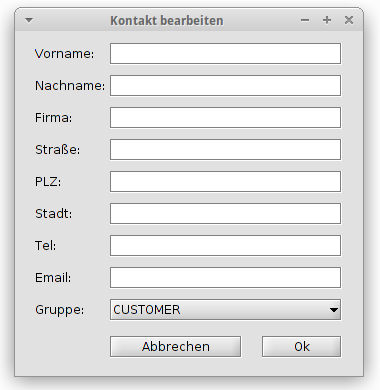
\includegraphics[width=\textwidth]{Bilder/Sib_EditContact_Frame.png}
\caption{Kontaktdaten anzeigen und verändern}
\label{fig:sibedit}
\end{figure}

Zuletzt fehlt noch die Möglichkeit, dass der Nutzer einen Kontakt aus einer Liste von Kontakten auswählen kann,
 sprich auf das Ergebnis einer Suchanfrage reagieren kann.
Das hier zu implementierende SIB benötigt also einen Parameter in Form einer Liste von \lstinline{Contact}-Objekten.
Auf der anderen Seite muss das \lstinline{Contact}-Objekt zurückgeliefert werden, welches der Nutzer ausgewählt hat.
Ähnlich zu vorherigen SIBs, sind diese Parameter als \lstinline{ContextKey} realisiert.
Das SIB liest die Kontaktliste aus dem Ausführungskontext und befüllt ein entsprechendes Fenster.
Nachdem der Nutzer einen Kontakt ausgewählt hat, werden die Daten entsprechend in den Kontext geschrieben.
Es wurden die Branches \emph{ok} (Eingabe beendet), \emph{cancel} (Eingabe abgebrochen) und \emph{error} (s.o.) definiert.

%Abbildung Choose
%\usepackage{graphics} is needed for \includegraphics
\begin{figure}[h!t]
  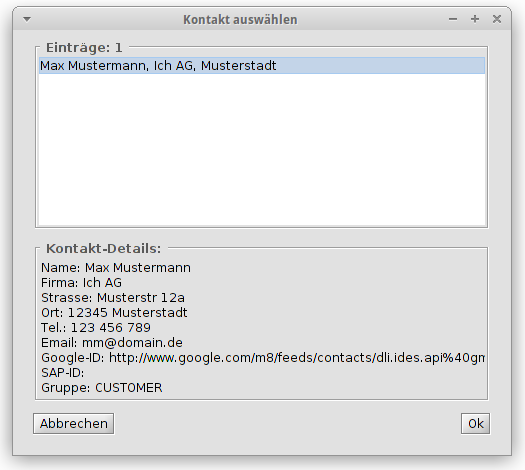
\includegraphics[width=\textwidth]{Bilder/Sib_ChooseContact_Frame.png}
  \caption{Einen Kontakt aus der Liste der Suchergebnisse auswählen}
  \label{fig:sibchoose}
\end{figure}

Um der Konvention von jABC zu folgen, wurde noch ein weiteres SIB implementiert.
In jABC ist es üblich ein sogenanntes \lstinline{Put}-SIB zu verwenden, wenn eine Variable eines bestimmten Typs im
 Ausführungskontext erzeugt wird.
Zu diesem Zweck startet das Prozessmodell mit einem SIB namens \lstinline{PutContact}.
Es erzeugt eine Instanz der \lstinline{Contact}-Klasse im Ausführungskontext, welche im Verlauf der Modellausführung
 verändert wird, bis ihr Inhalt zum Schluss dem Google-System hinzugefügt wird.
	
\FloatBarrier
\subsubsection{Besonderheit der GUI-SIBs}
Eine Besonderheit bei der Implementierung von SIBs ist die Benutzung von Komponenten des Swing-Frameworks.
Üblicherweise werden die erzeugten Fenster in einem separaten Thread gestartet, was den Effekt zur Folge hat, dass nach
 Erzeugung des Fensters die \lstinline{trace()}-Methode nicht auf Eingaben wartet, sondern weiter ausgeführt wird.
Während der Nutzer seine Eingabe noch nicht einmal begonnen hat, ist jABC mit der Ausführung der \lstinline{trace()}-Methode
 schon fertig.

Als Lösung des Problems bot sich die Java-eigene Möglichkeit zur Thread-Synchronisation mittels eines synchronized-Blockes an.
Eine exemplarische Verwendung zeigt \autoref{lst:sibsynchro}.

\javalstset{...}{lst:sibsynchro}
\begin{lstlisting}[float=h!t]

\end{lstlisting}
% synchro listing %

In diesem Listing ist der synchronized-Block der \lstinline{trace()}-Methode zu sehen.
Nachdem der Swing-Frame erzeugt wurde, dient jener als Synchronisationsobjekt.
Nachdem der \lstinline{synchronized}-Block betreten wurde, wird in \lstinline{trace()} die Methode \lstinline{wait()} aufgerufen.
An dieser Stelle stoppt die Ausführung von \lstinline{trace()}, bis das entsprechende Gegenstück, die Methode \lstinline{notify()},
 auf dem Synchronisationsobjekt aufgerufen wurde.
Dies geschieht innerhalb der ActionListener der verwendeten Buttons.
Wenn der Nutzer mit der Eingabe der Daten oder der Auswahl des Kontakts fertig ist, signalisiert er dies mit einem
 Klick auf einen Button.
Es wird der entsprechende \lstinline{ActionListener} des Buttons aufgerufen, welcher wiederum innerhalb eines
 \lstinline{synchronized}-Block die Methode \lstinline{notify()} aufruft und anschließend das Fenster schließt.

Die wartende \lstinline{trace()}-Methode wird daraufhin weiter ausgeführt und kann über geeignete Klassenvariablen
 des Frame-Objektes die Eingaben des Nutzers abfragen und in den Ausführungskontext schreiben.
\FloatBarrier
\subsubsection{Die JAVA-Laufzeitumgebung in jABC}	
Eine weitere Besonderheit hat sich während des Projektes zufällig ergeben.
Um das Zusammenspiel von Konnektoren und GUI-Elementen effizient zu testen, wurde auf die Ausführung der
 Komponenten im jABC zunächst verzichtet.
Erst zum Ende des Projektes wurden die Komponenten mittels ihrer zugehörigen SIBs in jABC getestet.
Es zeigte sich ein Fehler während der Ausführung, welcher außerhalb von jABC nicht aufrat.
Die geworfene \lstinline{Exception} ließ vermuten, dass bestimmte Bibliotheken innerhalb der Ausführung von jABC nicht
 gefunden werden konnten.
Unter Verwendung des selben Quellcodes außerhalb von jABC zeigte sich dieser Fehler jedoch nicht.
Dies legt die Vermutung nahe, dass die zur Laufzeit existierende Java-Umgebung in Form der Java-Virtual-Maschine (JVM)
 in beiden Szenarien nicht gleich ist.
Einige Bibliotheken werden innerhalb von jABC unter anderen Paketpfaden referenziert, als es außerhalb der Fall ist.
Zu diesem Zweck mussten die Eigenschaften der JVM im jABC manuell verändert werden. Dies ist in Listing \ref{lst:sibworkaround}
 zu sehen.

\javalstset{Workaround}{lst:sibworkaround} 
\begin{lstlisting}[float=h!t]

\end{lstlisting}

% Listing system.setproperty %

Auch wenn die Veränderung der Laufzeit-Eigenschaften das Problem behoben haben, so ist doch generell von dieser Praxis abzuraten.
Denn die veränderten Eigenschaften bleiben auch noch nach der Modellausführung im jABC bestehen, da jABC selbst ein Java-Programm
 ist und zur Ausführung von Modell die JVM des Programms verwendet wird.
Die Ausführung anderer Modelle im Anschluss an jenes dieses Projektes kann also beeinträchtigt oder im schlimmsten Fall gar
 nicht erst möglich sein.
\FloatBarrier